%!TEX root = ../template.tex
%%%%%%%%%%%%%%%%%%%%%%%%%%%%%%%%%%%%%%%%%%%%%%%%%%%%%%%%%%%%%%%%%%%%
%% chapter3.tex
%% NOVA thesis document file
%%
%% Chapter with a short latex tutorial and examples
%%%%%%%%%%%%%%%%%%%%%%%%%%%%%%%%%%%%%%%%%%%%%%%%%%%%%%%%%%%%%%%%%%%%

\typeout{NT FILE chapter3.tex}%

\makeatletter
\newcommand{\ntifpkgloaded}{%
  \@ifpackageloaded%
}
\makeatother


\chapter{Analysis and System Architecture}
\label{cha:analysis}

In order to explore the impact of portals with continuous previews on \glsfirst{VR} navigation and \glsfirst{UX}, we developed four portal variants 
for evaluation in a user study. To support this development and study, a functional system was required. This chapter explores the design and concepts 
necessary for the creation of said system, establishing the foundation for addressing the Objectives and Research Questions outlined in 
Section~\ref{sec:objectives-and-researh-questions}.

\todo{Dar um resumo do que será falado.}

\section{Requirements}
\label{sec:requirements}


This research proposes the study of four \gls{VR} locomotion techniques based on portals in a Non-Euclidean environment examining its impact on 
navigation and \gls{UX}. It was essential to create a \gls{VR} experience within a Non-Euclidean \glsfirst{VE} that relied on the use of portals 
for locomotion, paired with a suitable simple task that demanded users' to navigate throughout the environment using the developed techniques.

The system was designed to create a \gls{VE} that supports natural walking and hand-tracking to maximize feelings of presence and immersion. Users 
perceive the world through a \glsfirst{HMD} that is simultaneously tracking their movement in the physical environment, as well as their hands 
through the cameras present on the face of the \gls{HMD}. The hand-tracking is used for interacting with the \gls{VE}, whether it be for interacting with the 
portals, allowing users to navigate, or to interact with elements of the study's task.

During the conceptualization of the portals to be developed a study was conducted comparing Teleporting with Walking with Portals in 
\gls{VR} which led to the submission and publication of an article for ACM Multimedia 2025~\cite{}\todo{já dá para citar o artigo?}.
The study took place in a virtual apartment, where participants were first asked to explore and then to complete an object fetch-quest, 
using one technique at a time. The study identified a key trade-off between the portal's distance from the wall and the clarity of the 
next-room preview. To ensure that users can safely turn 180 degrees after passing through without leaving the tracked play area, the portal 
must be positioned at least 60–80 centimeters away from the virtual wall. However, this requirement introduces an awkward “dead space” and 
creates a design conflict. Placing the portal closer to the wall conserves physical space but limits the preview to little more than 
a wall and a narrow strip of floor. In contrast, positioning the portal further away offers a broader, more informative view of the next room, 
but does so at the expense of valuable room space and at the risk of appearing unnatural, like a floating frame. With this in mind, our solution 
required to approach these limitations.

In summary, the main requirements of our solution are as follows:

\begin{itemize}
  \item Allow users to navigate the entirety of the \gls{VE} solely by naturally walking in a limited physical tracking space (similar to 
  the available space of common \gls{VR} users, thus around 2.4 x 2.2 meters\cite{Azmandian2015, Liu2018b}).
  
  \item Include variants of portal techniques that address the limitations caused by their placement and lack of preview.
  
  \item Include a common portal technique as a baseline for comparison with the variant techniques.

  \item Support interaction with the \gls{VE} through hand-tracking, for interacting with portals and the task to be performed during the study.
 
  \item Include a task that incentivizes users to explore the entirety of the \gls{VE}.
  
  \item Task design should be simple enough to be repeated with different locomotion techniques without introducing task-specific biases. 
  
\end{itemize}

\section{Case Study}
\label{sec:case-study}

A case study was designed in order to address the aforementioned requirements and investigate the proposed research questions. 
With the goal of studying the usability of portal variants with continuous previews as \gls{VR} locomotion techniques in a small 
physical space (about 2.5 x 2.5 meters), an interior \gls{VE} with a self-overlapping architecture was chosen as the experimental 
environment.

As such, the case study was designed as a museum experience, serving as an interior \gls{VE} that can be contained in a constrict physical tracking 
space through the use of a self-overlapping non-Euclidean virtual space. This setting also permits a more natural selection of exploratory  and 
immersive tasks that rely on the use the developed locomotion techniques. The chosen tasks were associated with exposition items and artworks 
present in the museum, taking the form of small quiz questions that, once answered, reveal a curious fact about the artwork, gearing users 
toward exploring the whole environment and feel present in the experience.

The multiple rooms of the \gls{VE} should be connected through the portal techniques, creating the self-overlapping architecture. In the interest 
of analyzing the experience from each portal separately, the environment should be divided in as many sections as the number of portal variants, one 
for each variant, that should have the same room layout and the same tasks in order to ensure the validity of comparisons.

Throughout the case study users wear a \gls{HMD} and naturally walk around the physical environment of 2.5m x 2.5m. To interact the \gls{HMD} 
should capture users' hand movements through hand-tracking. Hand-tracking was opted instead of controllers in order to maintain the highest levels 
of presence possible. All users should experience all portal variants in order to accomplish a within subject comparison, hence users should 
sequentially experience all the sections of the museum.

The procedure for the case study follows a structured sequence of tasks that is repeated in each section. 
First, participants explore the assigned museum section using one of the portal variant techniques, interacting with the exhibited items. 
Once the section has been fully explored and participants have experienced the locomotion technique, participants are then tasked to evaluate the 
navigation technique.
Afterward, participants proceed to the next section, where the same sequence is repeated with a different portal variant.

With this case study it is possible to meet the requirements necessary to investigate the research questions in a controllable environment, 
ensuring that the constraints of a limited physical space are respected while allowing systematic evaluation of the proposed portal variants. 
By employing a within-subject design, a uniform task structure, and consistent room layouts, the study ensures comparability across techniques 
and supports the collection of reliable data on usability, presence, and user experience.

\section{Architecture and Technologies}
\label{sec:architecture-and-technologies}

To develop the case study, it was necessary to define an architecture that could address the aforementioned requirements and research questions.
The proposed system and the tools used to create it are presented in Figure~\ref{fig:architecture}, divided by their function: input, processing 
and output.

A foundational \gls{VR} application was required to construct the \gls{VE}, which in turn necessitated the use of a game engine. \textbf{Unity} 
was the chosen tool for creating the application, as it is widely adopted in both industry and research for \gls{VR} development and provides 
a wide range of assets and plugins. To further abstract and simplify the integration with \gls{VR} devices, we resort to the \textbf{OpenXR SDK}, 
providing and additional layer of abstraction that enables compatibility with a wide range of \gls{VR} devices.

Using the \textbf{Unity} game engine with the imported \textbf{OpenXR Plugin} the process of creating an interactive 3D \gls{VE} was simplified and streamlined, 
since these create the possibility of composing the environment with \textbf{C\# scriptable objects}. This allowed the implementation of the portal 
techniques and the UI elements needed for the study's tasks, as well as a streamlined integration of these implemented objects into the \gls{VR} 
application. The \textbf{XR~Interaction~Toolkit~(XRI)} and \textbf{XR~Hands} Unity packages were imported as Unity packages, further streamlining 
the implementation of the interactable elements of the application, by providing a high-level framework for interactions and 
hand-tracking support respectively.

Finally, to receive the inputs that affect the interactive \gls{VR} application and display the effects of said interactions, a \gls{HMD} was 
needed. We opted for the use of the \textbf{Oculus Quest~3} \gls{HMD}, as it supports the most desired functionalities for the proposed 
case study: inside-out tracking for tracking the users' position in the \gls{VE}, hand-tracking via its front-facing cameras for more 
immersive interaction, and a high-resolution display for visualizing the \gls{VE}.

By combining these tools and structuring this architecture it is possible to meet the requirements of this case study: create a self-overlapping 
\gls{VE} using different portal techniques, explorable through natural walking and interactable through hand-tracking technologies.

\begin{figure}[t]
    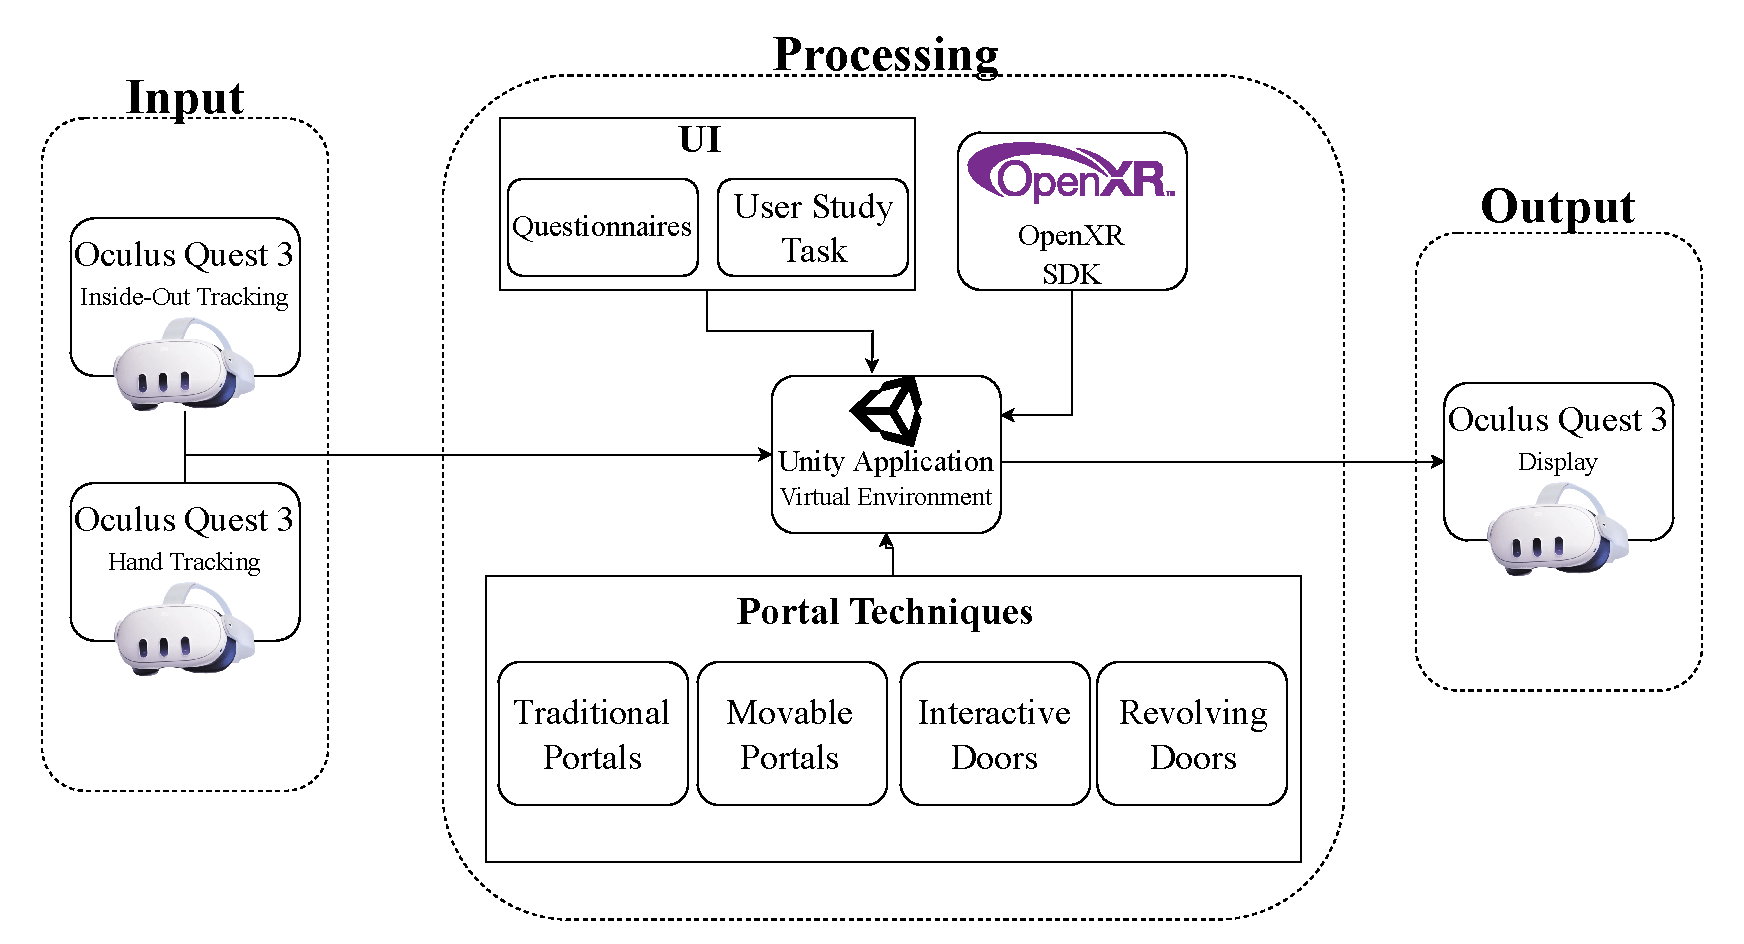
\includegraphics[width=\textwidth]{NOVAthesisFiles/Images/schemes/architecture-overview.drawio.pdf}
    \centering
     \caption[Overview of the architecture of the solution.]
     {Architecture overview.}
     \label{fig:architecture}
\end{figure}


\section{Preliminary Experiments}
\label{sec:preliminary}

\todo{Complete according to space}

\section{Portal Designs}
\label{sec:portal-design}

This study aims to explore and study variants of \gls{VR} locomotion techniques based on natural walking with portals. As such, we propose three 
portal implementations that address the limitations of commonly used portals in \gls{VR} research and applications, namely the lack of a proper 
preview when portals are placed closed to the limits of a \gls{VE} and the unnaturalness caused when portals are placed further away from these 
limits.

This section presents the design choices underlying the four portal techniques examined in our user study: Traditional Portals, serving as the baseline 
condition representing the commonly used portals in \gls{VR} research, and the three proposed variants — Movable Portals, 
Interactive Doors, and Revolving Doors.

\subsection{Traditional Portal}
\label{sec:trad-portal-design}

Our baseline condition represents the conventional approach to portals in \gls{VR}, commonly seen in both commercial applications
and academic research. Appearance-wise a door frame-shaped portal was chosen, both for its similarity to those used in prior 
research and for its association with the familiar real-world concept of doors.

The preview capabilities of this type of portal are, thus, the same as the ones commonly found in \gls{VR} research and applications. As such, 
it is possible to evaluate the limitation of this type of preview when used in \gls{VR} applications that resort to natural walking as a means 
of locomotion when compared to the proposed portal variants. Figure~\ref{fig:trad-portal-preview} represents the core challenge of traditional portals 
addressed by this work.

\begin{figure}[t]
    \centering
     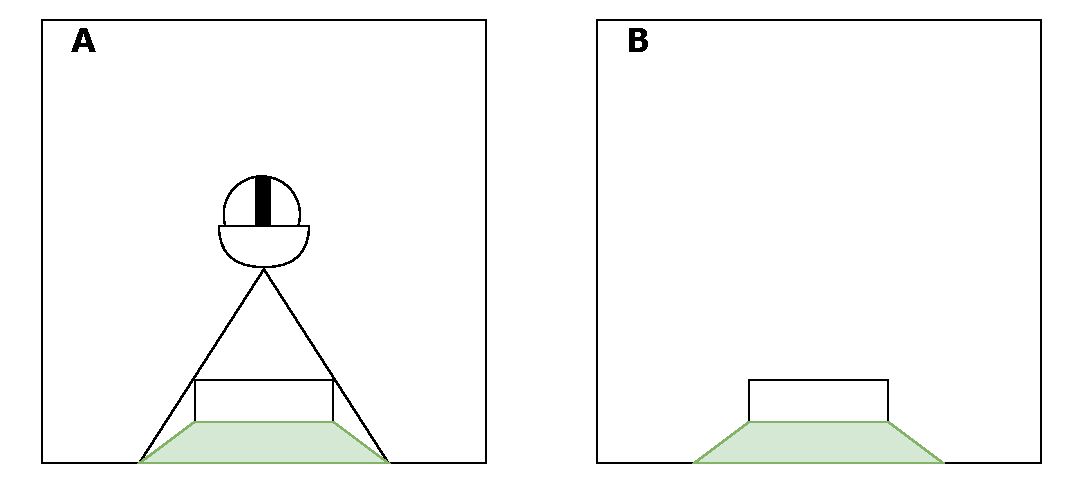
\includegraphics[width=.75\textwidth]{NOVAthesisFiles/Images/schemes/trad-portal-preview.drawio.pdf}
     \caption[Representation of the limitation of Traditional Portal previews.]
     {Representation of the limitation of Traditional Portal previews: The closer the portal is to the limits of the \gls{VE} the 
     observable preview diminishes, often revealing only a narrow segment of the connected space.}
     \label{fig:trad-portal-preview}
\end{figure}

\begin{figure}[b]
    \centering
     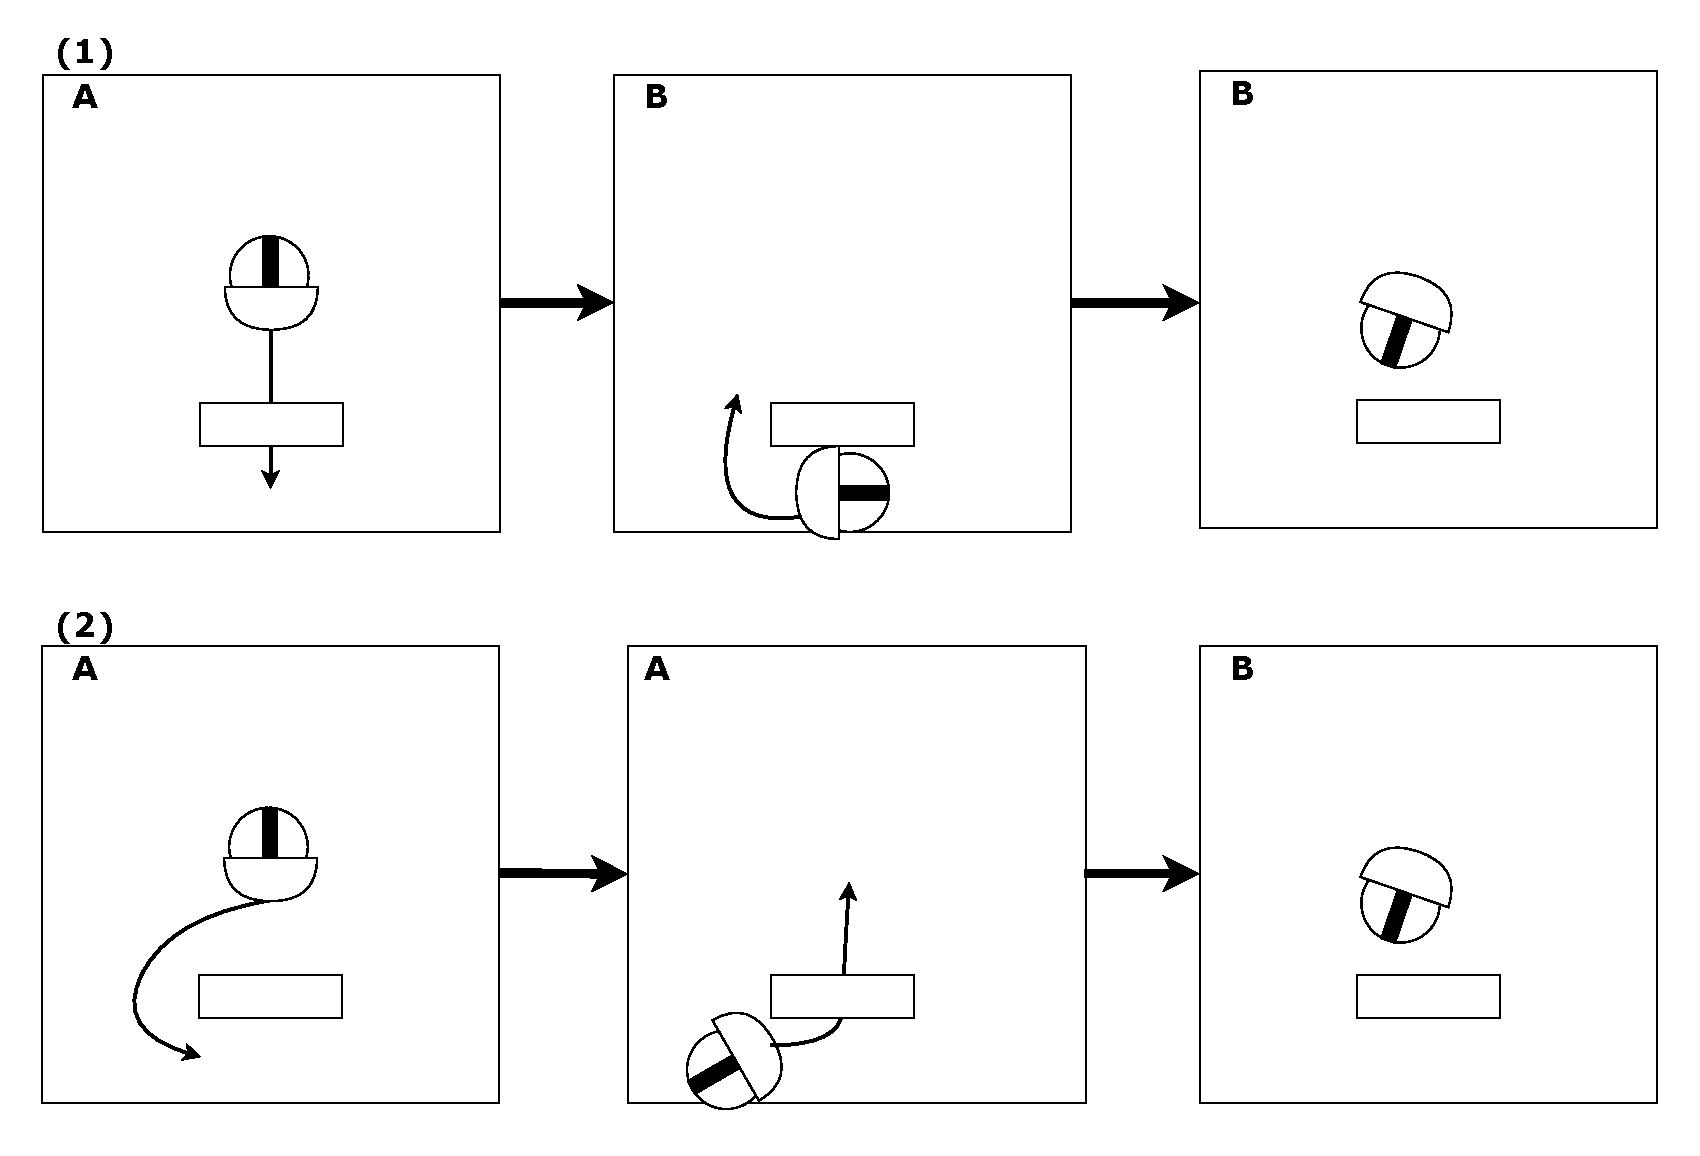
\includegraphics[width=.75\textwidth]{NOVAthesisFiles/Images/schemes/trad-interaction.drawio.pdf}
     \caption[Interaction design of the Traditional Portal.]
     {Two possible approaches to transition using Traditional Portals. (1) Users can go directly through the portal, with a minimal preview 
     before transition, (2) or move around the portal to first get a proper preview of the room before transitioning.}
     \label{fig:trad-portal-interaction}
\end{figure}

The level of interaction with this portal is minimal, as to use it the user must simply pass through the frame. 
As such, since the limits of the \gls{VE} correspond with the limits of the physical environment, these portals should be placed within a 
distance of circa 80cm \todo{check value} from the borders of the \gls{VE}, so that users don't reach the physical limits of the tracking space.
This portal placement further explores the limitation of these portals, as to use them users have to either: (1) go through the portal with a 
minimal preview and move around it in the destination room, (2) or move around the portal in their current room, obtain a better preview of the 
destination room and finally go through the portal (see Figure~\ref{fig:trad-portal-interaction}). Either of these options, however, causes the user to complete a 
180-degree turn, redirecting them towards the center of the available physical tracking space.


\subsection{Movable Portal}
\label{sec:mov-portal-design}

The Movable Portal's design addresses the wall clearance issue by allowing users to dynamically create the necessary space for transition. The main 
goal of this design is to provide user's a higher sense of control over the amount of space portals take, while additionally providing a better 
preview of the rooms that these portals are connected to. This is achieved by having the portal initially placed against the wall, with a reversed 
preview that renders the connected room as if it was positioned in a continuous space, instead of a self-overlapped space. Users can then move 
the portal when they wish to go through them, reversing the preview to the same manner it is rendered on Traditional Portals.

Thus, the designed interaction with this portal would go as follows:

\begin{enumerate}
  \item Portal is against the wall, rendering a continuous preview into the connected room.
  \item After accessing their destination, the user decides to go through this portal.
  \item The user grabs the portal using their virtual hands. As they do, a valid placement area is rendered, indicating the user where they may 
  place this portal.
  \item After choosing their pretended placement, the user lets go of the portal. If the portal is positioned within the bounds of the valid area, 
  it is placed and the preview is reverted according to the self-overlapped architecture. Otherwise, the portal reverts back into its original 
  position against the wall with a continuous preview.
  \item If the portal is correctly placed, the user may seamlessly transition to the connected space by moving through the portal.
\end{enumerate}

Although the main goal of this design is to empower users with a strong sense of control, the valid area was created in order to have a failsafe 
measure against portals overlapping with other objects in the environment. It was also necessary to reverse the preview when the portal is place, 
since if the preview was kept, the transition would cease to be seamless, as the preview would not correspond to the position the user would be 
transitioning to. 

The Movable Portal's appearance was designed similarly with the Traditional Portal's design, being presented as an empty door-frame. However,
it differs itself from the Traditional Portals by having a handle-like affordance to signal users that the portal should be grabbed in order to 
complete the interaction.

\begin{figure}[t]
    \centering
     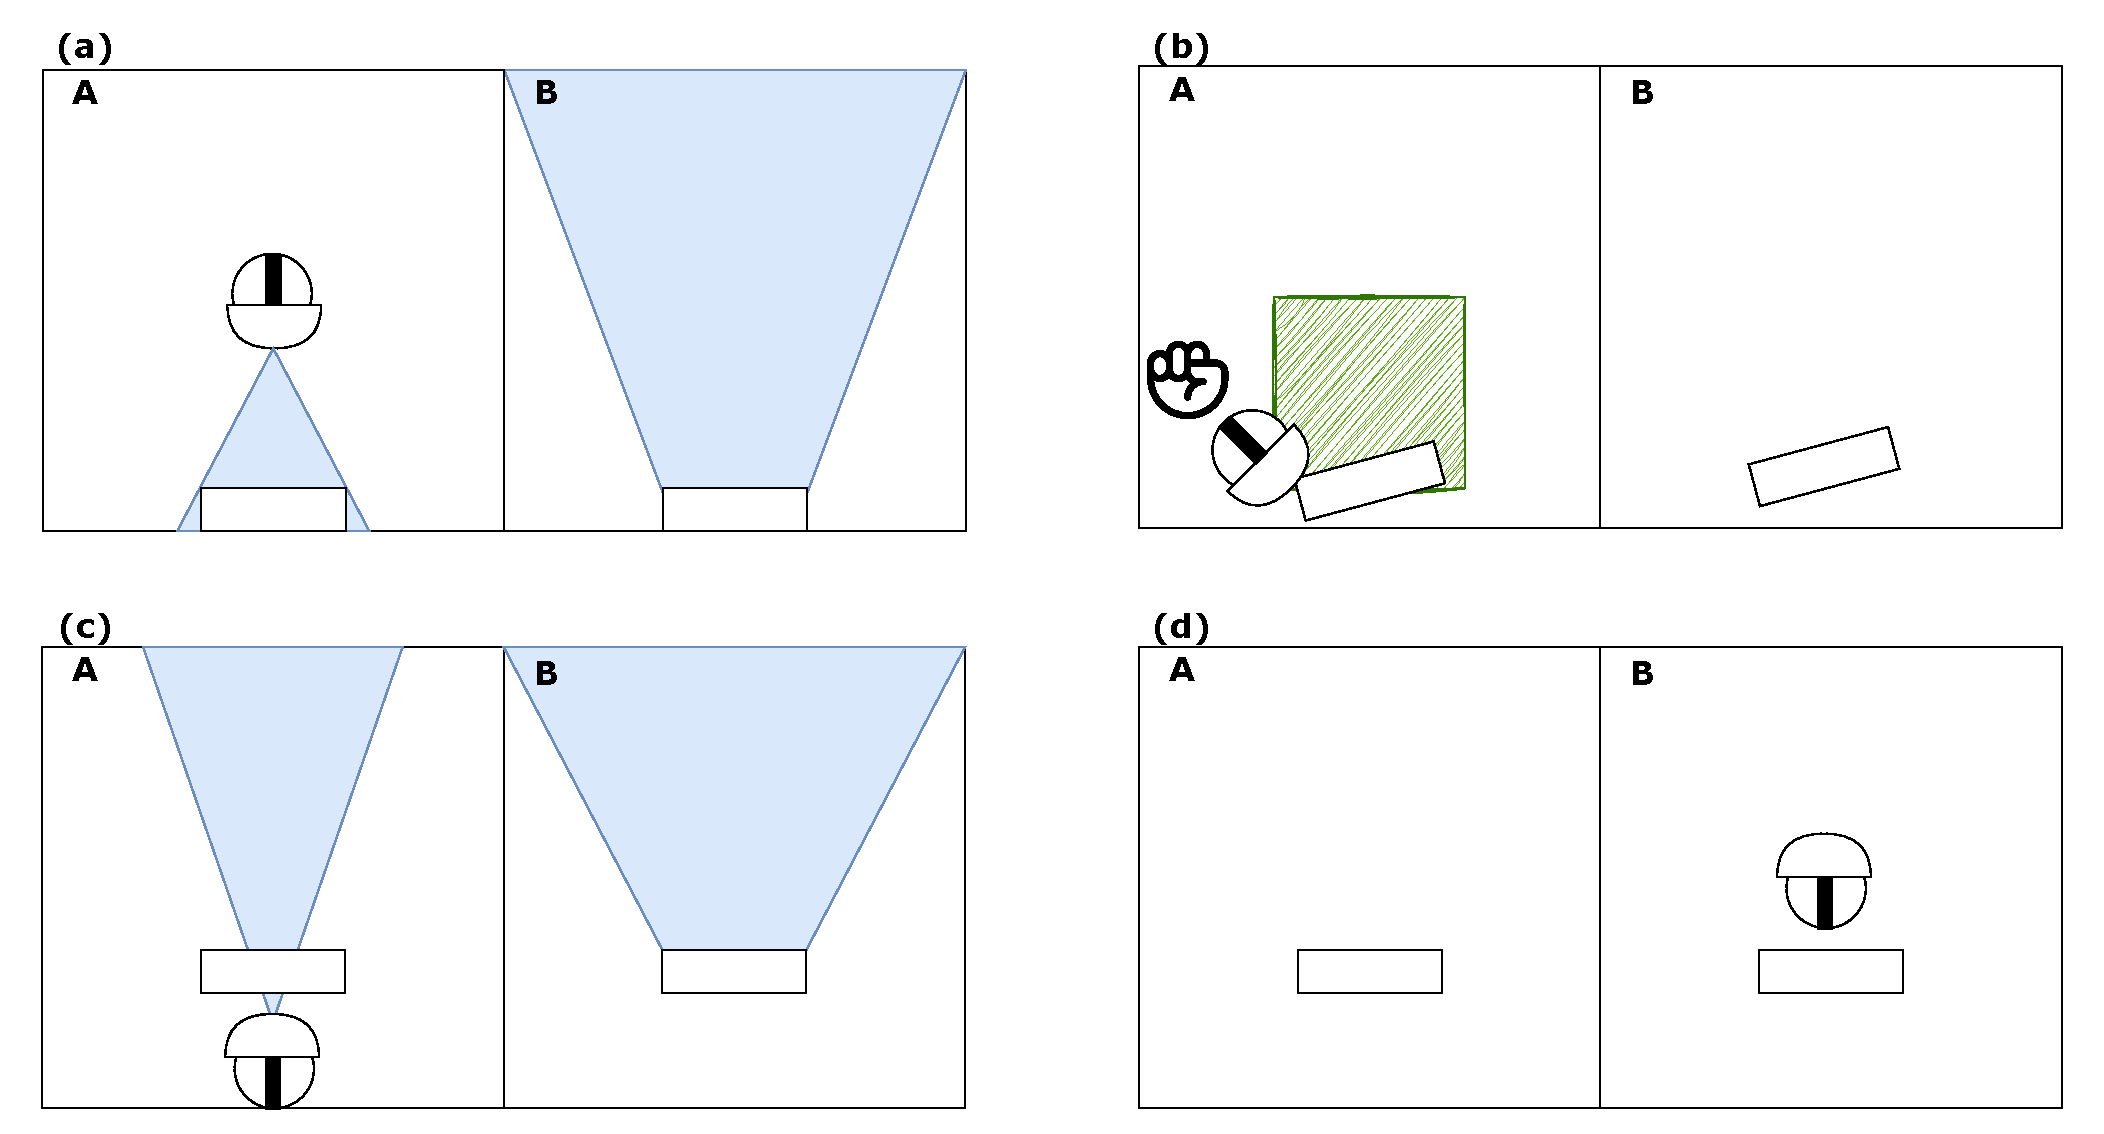
\includegraphics[width=.9\textwidth]{NOVAthesisFiles/Images/schemes/mov-interaction.drawio.pdf}
     \caption[Interaction design of the Movable Portal.]
     {Interaction design of the Movable Portal: (a) At the start of the interaction the portal is placed against the wall with a 
     reversed preview for a continuous appearance. (b) The user can then grab the portal with their virtual hands, which will prompt 
     a valid area to render. The 
     associated portal will follow the placement of the portal. (c) The user can then let the portal go within the bounds of the valid 
     area, placing the portal and reverting the preview. (d) The user can then go through the portal.}
     \label{fig:mov-portal-interaction}
\end{figure}

\subsection{Interactive Door}
\label{sec:int-door-design}

The Interactive Door's design prioritizes naturalism by modeling the portal after a familiar real-world object: a door. The main goal of this design 
is to maximize immersion and intuitive use by leveraging users' everyday experience with doors, while simultaneously providing a reliable solution 
to the wall clearance issue. 

Initially, the Interactive Door is transparent, offering a continuous preview of the adjacent room. This choice supports exploration by allowing 
users to perceive the contents of the next room before committing to interaction. As the user approaches, however, the door becomes opaque, 
prompting users to interact with it in order to complete the transition. After opening the door, similarly to the Movable Portal, the preview 
reverses to correspond with the self-overlapping architecture.

The interaction sequence can be summarized as follows:

\begin{enumerate}
  \item The door is placed against the wall, transparent, rendering a continuous preview into the connected room.
  \item As the user approaches the door, its surface becomes opaque, signaling that interaction is required.
  \item The user reaches out with their virtual hand, grabs the handle, and performs a swinging motion to open the door, closely mimicking 
  real-world behavior.
  \item As the door swings open, the portal accompanies the door-frame. The preview is discreetly reversed.
  \item Once the door is sufficiently open, the user may seamlessly transition into the connected room by walking through the doorway.
\end{enumerate}

This interaction design achieves several objectives simultaneously. Firstly, the rotation of the door provides the necessary clearance from the 
virtual wall, ensuring that users are redirected into their available space by turning in a 90-degree angle. Secondly, the portal's door-like 
appearance is designed to convey a more natural and easy interaction, by emulating the act users do on a daily basis in the real world. 
Finally, the opacity change permits to covertly change the preview of the portal, allowing the portal to render a continuous preview when 
against the wall, and then rotate to match the self-overlapped space when opened.

\begin{figure}[t]
    \centering
     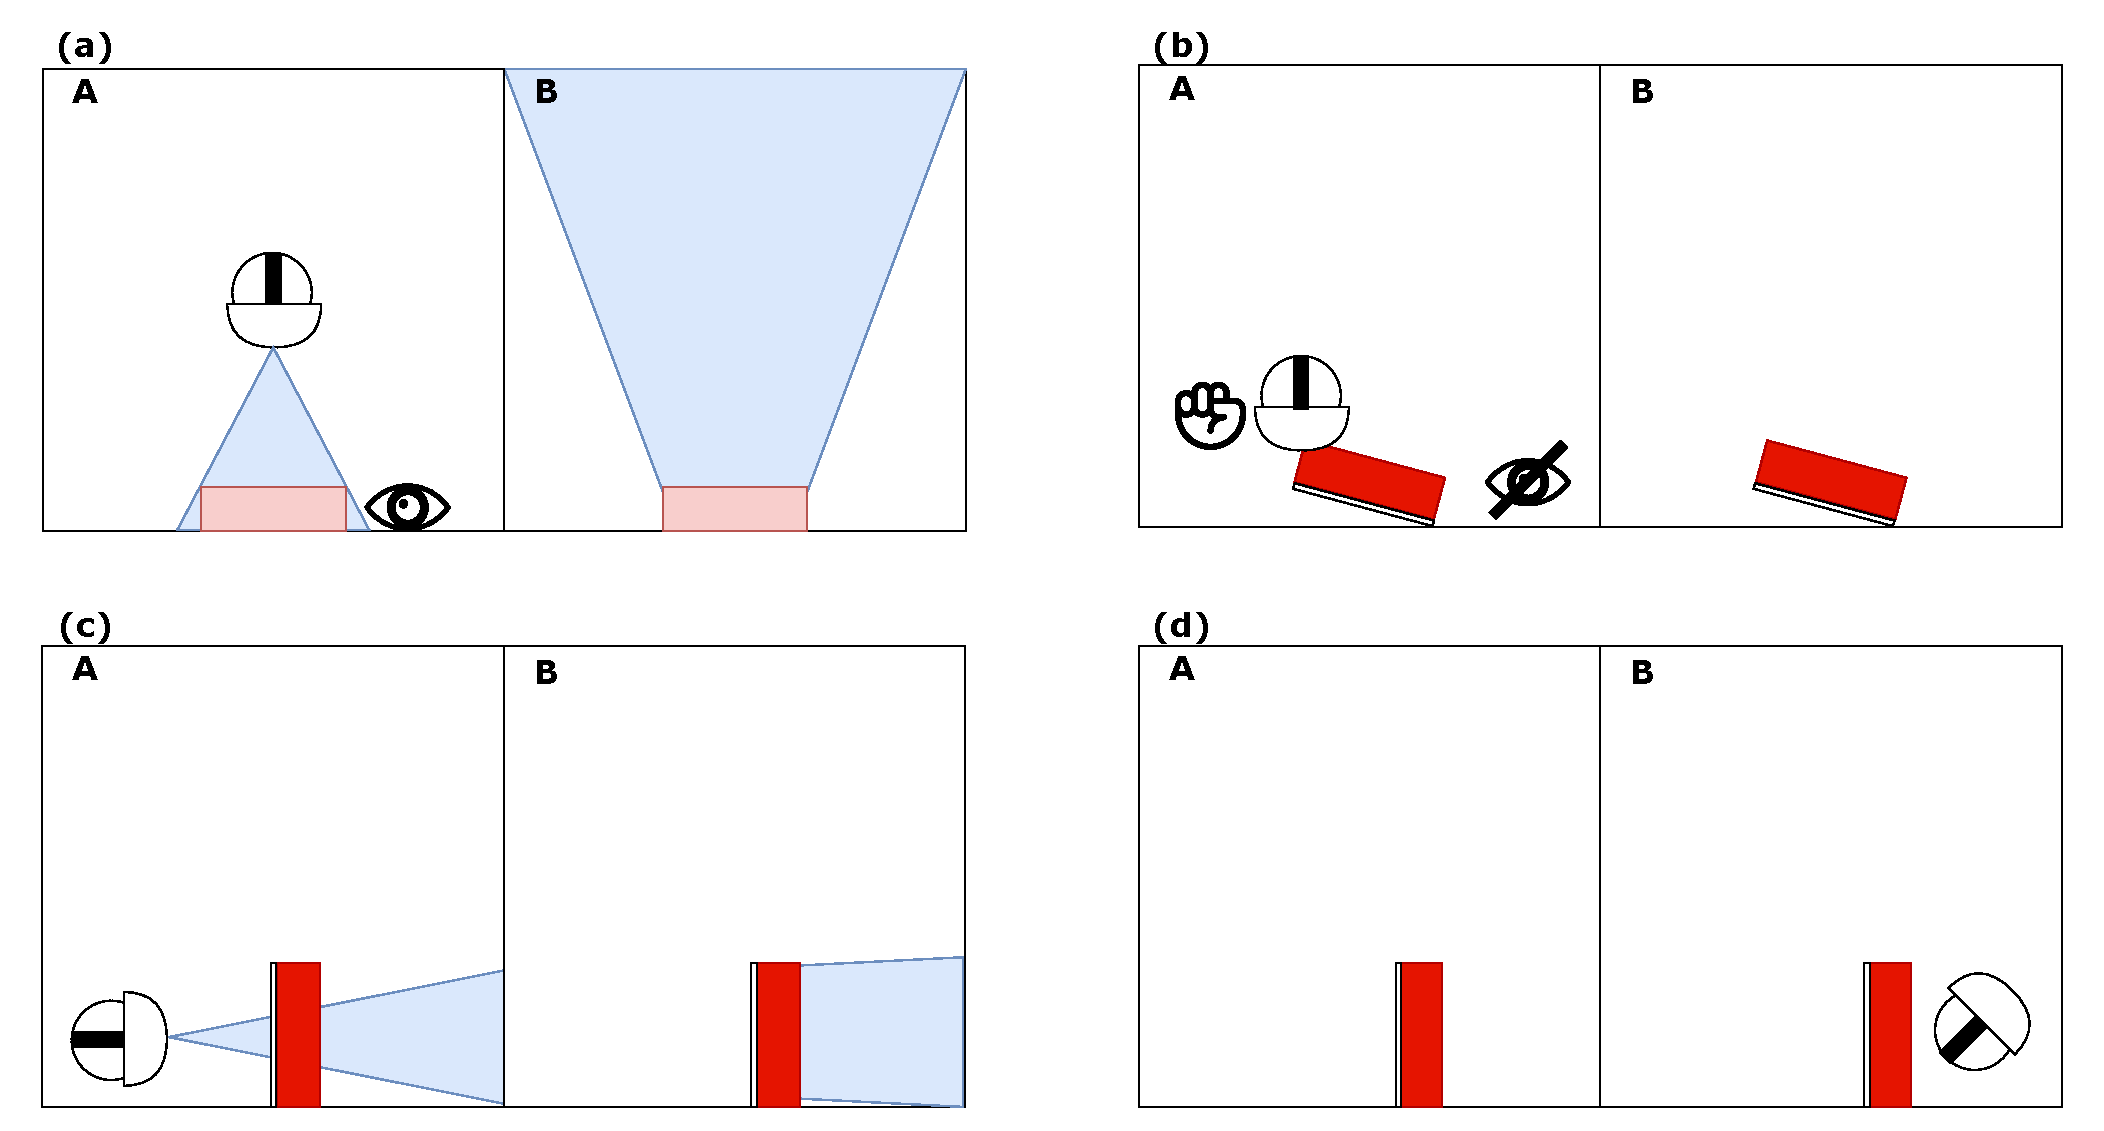
\includegraphics[width=\textwidth]{NOVAthesisFiles/Images/schemes/door-interaction.pdf}
     \caption[Interaction design of the Interactive Door.]
     {Interaction design of the Interactive Door: (a) From a distance the material of the door has low opacity, being transparent enough to 
     reveal the portal behind it with a reversed continuous preview. (b) As the user approaches the door it becomes more opaque. When fully 
     opaque, the user can grab the handle and swing the door open. (c) The door will open to a maximum of 90\textdegree, with the portal accompanying 
     it throughout the motion. (d) The user can go through the portal to reach the connected room.}
     \label{fig:door-portal-interaction}
\end{figure}

\subsection{Revolving Door}
\label{sec:rev-door-design}

The Revolving Door's design explores a more continuous and guided form of transition, employing the metaphor of a revolving door to manage both 
the physical and virtual reorientation of users. Similarly to Interactive Door, the appearance of the Revolving Door changes dynamically based 
on proximity. From a distance, the door is transparent, allowing the user to preview the next room through a portal that renders a continuous preview 
to the next room, and as the user approaches, the door becomes opaque, concealing the preview and prompting direct physical interaction.  

\begin{figure}[t]
    \centering
     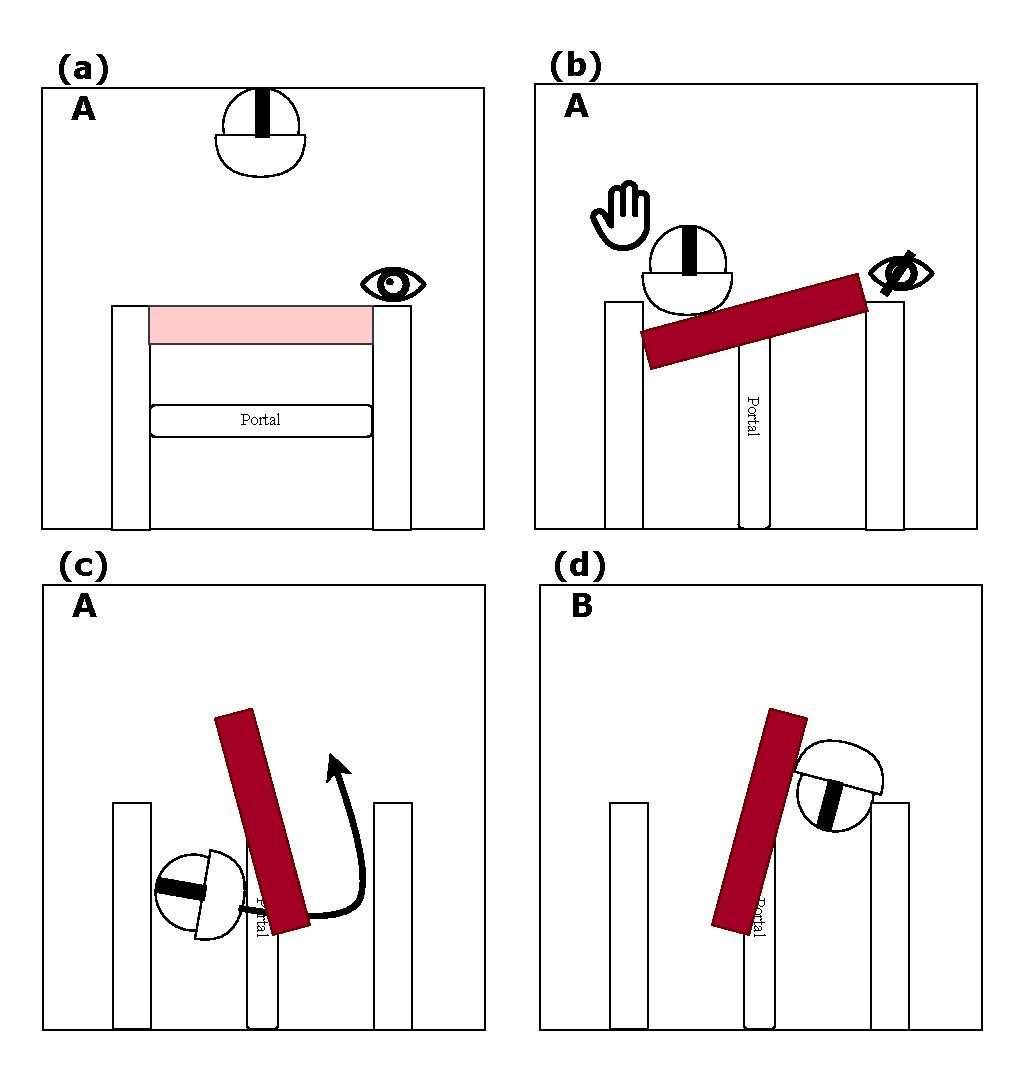
\includegraphics[width=.6\textwidth]{NOVAthesisFiles/Images/schemes/rev-interaction.pdf}
     \caption[Interaction design of the Revolving Door.]
     {Interaction design of the Revolving Door: (a) From a distance the material of the door has low opacity, being transparent enough to 
     reveal the portal behind it with a reversed continuous preview. (b) As the user approaches the door it becomes more opaque. When fully 
     opaque the portal rotates 90\textdegree and reverts its preview. (c) As the user pushes the door, the door guides them to complete 
     a 180\textdegree turn and to pass through the now perpendicular portal. (d) The user emerges from the other side of the door in the connected 
     room.}
     \label{fig:rev-portal-interaction}
\end{figure}

The intended interaction sequence is as follows:

\begin{enumerate}
  \item The revolving door is integrated into the wall, initially transparent to provide a continuous preview of the adjacent room.  
  \item As the user approaches, the door becomes opaque, signaling that direct interaction is required.  
  \item The user steps into the door's compartment and begins pushing the door using their virtual hand.  
  \item As the door shifts to full opacity, the portal placed behind the door reorients by 90 degrees.  
  \item The physical motion of the door guides the user through a 180-degree turn, ensuring proper reorientation into the connected room.  
  \item During this movement, the user seamlessly passes through the perpendicular portal and emerges in the new space once the door has 
  completed its rotation.  
\end{enumerate}

Although in a different type of physical interaction, this design achieves the same objectives as the previous variants. 
Firstly, the revolving mechanism provides the necessary clearance from the virtual wall by guiding the user 
through a 180-degree turn, ensuring they are correctly oriented towards the available space. Secondly, the door's appearance is designed to 
foster a more natural and intuitive interaction, as it builds on users' familiarity with a real-world object. 
Finally, the opacity change permits the system to covertly adjust the 
portal's preview: from a continuous preview when the door is at transparent, to a rotated preview 
that matches the self-overlapped architecture as the door turns during the transition.


\section{Summary}
\label{sec:chap3-summary}

\todo{Completar de acordo como o ficar no fim. Aproveitar para dara uma revisão do texto completo para perceber se está coerente.}